\chapter{Results}
\label{chap:3}
\ChapterPageStuff{3}

\section{Preamble}
Introduction of the chapter.

\section{Logging mechanism}

\subsection{Obtaining the element of user-based event}\label{sec:ch2_ElementObtaining}
In \Cref{sec:ch2_webApplicationArchitecture} the user-based activity event will be use a \textit{HTTP request} to send to the server when the user interacted with an \textit{HTML element}. For the functional requirements activity type (F/R 1.5.3) and metadata (F/R 1.5.6) in \Cref{tbl:ch2_keyLoggingAttributes} the \textit{HTML element} needs to be obtained to get the element's tag and identification text. This can be difficult to obtain due to \textit{bubbling}\footnote{\textbf{Bubbling} is when an event happens on an element, it first runs the handlers on it, then on its parent, then up on other ancestors. \cite{EventBubbling}.} that may occur when searching for the element that the user specifically interacted with.\par In \Cref{fig:ch2_event_bubbling} is the event propagation example of a child element that has been clicked on which executes a DOM event. The event propagation consists of three phases~\cite{EventBubbling}:

\begin{itemize}
	\item \textit{Capturing phase:} The event propagates downwards to the targeted element that the user interacted with.
	\item \textit{Target phase:} The event reaches the targeted element to execute the DOM event.
	\item \textit{Bubbling phase:} The event bubbles up from the targeted element
\end{itemize}

\begin{figure}[!htb] % An h :here, t: top, b: bottom.
	\centering % cent the figure
	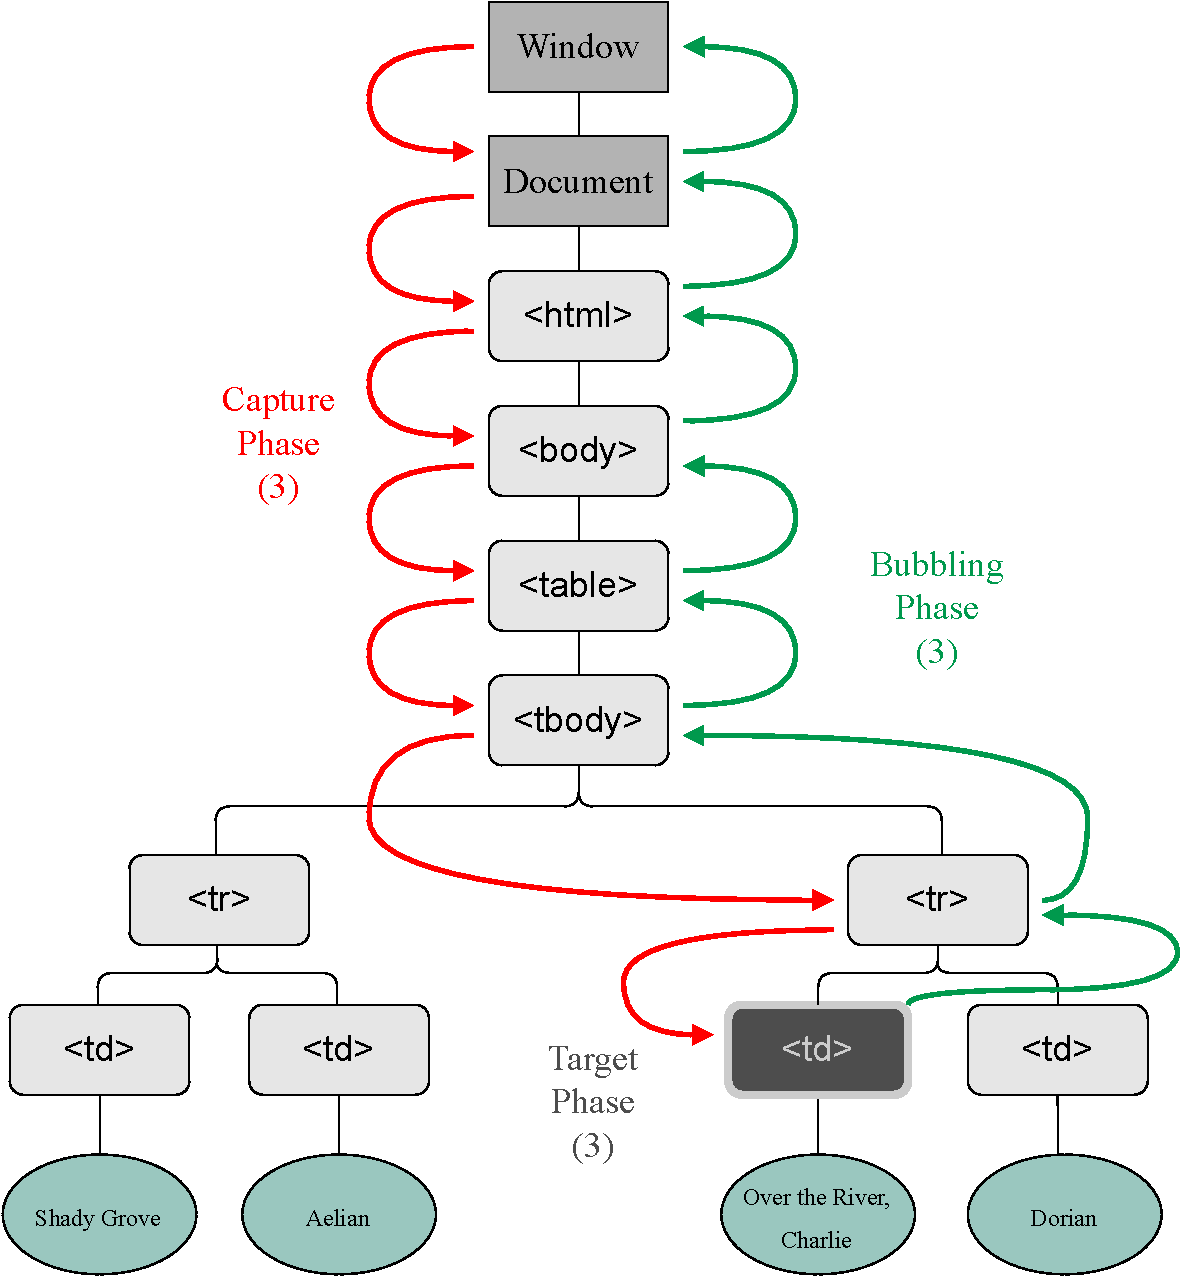
\includegraphics[width=0.6\textwidth]{Chapter2/event_bubbling/event_bubbling.pdf}
	\caption[JavaScript event propagation]
	{\textit{JavaScript event propagation~\cite{EventBubbling}}}\label{fig:ch2_event_bubbling}
\end{figure}

Capturing the targeted element may be difficult as some Web pages may have more complex HTML where the event propagation may sometimes not obtain the correct element information which the user interacted with. Another DOM event may have started during the initial element's event, therefore it is more accurate to obtain the targeted element by obtaining the last known element the user hovered over on the user interface.\par In \Cref{fig:ch2_element_event_capturing} is the flow diagram to capture the element user interacted with for the user-based activity log. This code segment will be initiated during the \texttt{beforeSend} operation of the \textit{AJAX request} to filter HTML elements by predefined allowed elements to use. Filtering the element tag names ensures that unwanted more complex elements or more basic elements that are not expected to be the initiator of the event will be used. \par If the Web location already changed or no element exists, the contents of the page might have already changed during the event propagation. The last known element that the user hovered on must be used as most likely might have been the element that the user interacted with. This will ensure there is always an element that has been detected and parsed with the request header in most UI changes.

\clearpage

\begin{figure}[!htb] % An h :here, t: top, b: bottom.
	\centering % cent the figure
	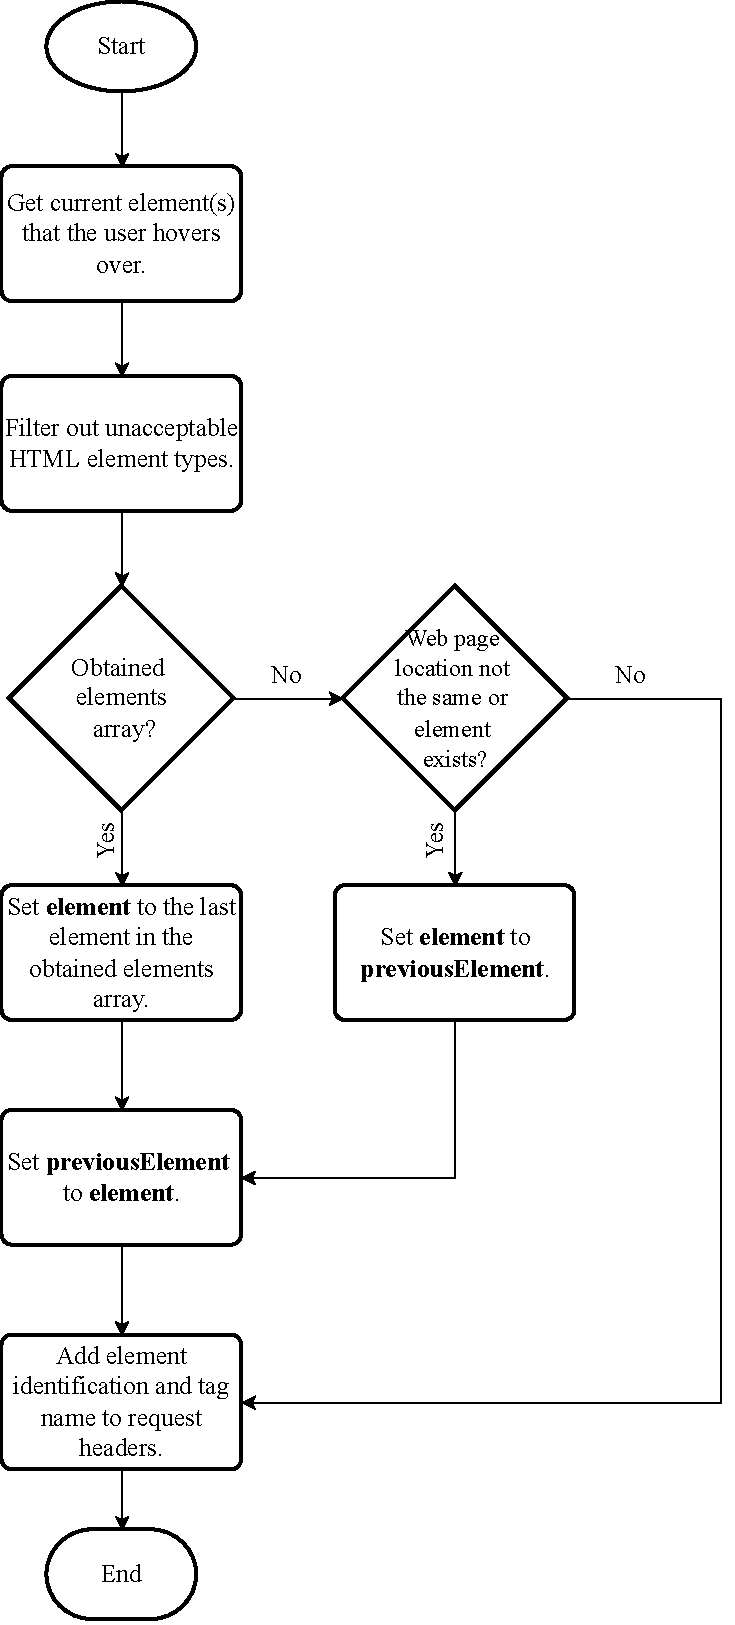
\includegraphics[width=0.5\textwidth]{Chapter2/element_capturing/element_capturing.pdf}
	\caption[HTML element capturing flow diagram]
	{\textit{HTML element capturing flow diagram}}\label{fig:ch2_element_event_capturing}
\end{figure}

\section{Utilisation analysis}


\section{Verification}\label{sec:ch3_verification}
Using the functional requirements defined in \Cref{sec:ch2_loggingMechanism,ch2:sec_system_utilisation_analysis} the system can be verified that it satisfies the system requirements in \Cref{tbl:ch2_verification}.

\begin{table}[!htb]
	\centering
	\caption[System requirements for verification]
	{\textit{System requirements for verification}}
	\label{tbl:ch2_verification}
	\begin{tabularx}{\textwidth}{|X|X|c|}
		\hline \textbf{Requirement} & \textbf{Methodology reference} & \textbf{Satisfied} \\
		\hline \textbf{User activity types} &  & \cmark \\
		\hline \textbf{Log attributes} & & \cmark \\
		\hline \textbf{Logging points} &  & \cmark \\
		\hline \textbf{Log extraction and visualisation} &  & \cmark \\
		\hline \textbf{System utilisation analysis} &  & \cmark \\
		\hline
	\end{tabularx}
\end{table}

\section{Conclusion}
